\documentclass{article}
\usepackage{iclr2027_conference,times}
\usepackage{amsmath,amssymb,graphicx,booktabs,microtype}
\usepackage{hyperref}
\usepackage{url}
\title{Does Memory Provenance Matter? Exact-Information Swaps Show Low Terminal Value Beyond Content}
\begin{document}
\maketitle
\begin{abstract}
Self-evolving agents convert prior trajectories into reusable memory, but a memory item can carry two distinct signals: actionable content and the process provenance of the trajectory from which that content was written. We ask whether success/failure provenance adds downstream value once actionable memory content is held fixed. We introduce an L0--L3 provenance-audit ladder separating observational association, outcome-conditioned writer effects, exact-information provenance exposure, and source-faithful transport. We then execute a prospective L2 experiment on MemRL/OSInteraction. A full 350-task source run yields 176 success-derived and 174 failure-derived memories; before any validation outcome, native retrieval supports 106/108 fresh dependency clusters and a disjoint utilization gate verifies behavioral memory use. On 32 frozen primary clusters with Qwen2.5-7B-Instruct, content-only memory succeeds on 15/32 tasks and the identical content plus truthful provenance succeeds on 16/32, giving $\Delta=+0.03125$, exact paired $p=1.0$, and a preregistered bootstrap 95\% interval $[0,0.09375]$. Provenance still changes first executable action in 9/32 clusters, indicating behavioral legibility without reliable terminal conversion. We then replicate the exact same source bank, retrieval/content/order, units, renderer, endpoint, and analysis with Meta-Llama-3.1-8B-Instruct. Its independent utilization gate passes strongly (8/8 memory-specific versus 5/8 placebo divergences), while the 32-pair terminal effect is exactly $0$ (two B-only and two A-only successes), with $p=1.0$ and interval $[-0.125,0.125]$. Neither model reaches the prespecified $|\Delta|\geq0.15$ relevance floor, and we do not pool them. Thus raw provenance is behaviorally available yet shows replicated low incremental terminal value beyond fixed content on this qualified substrate. This supports a bounded content-sufficiency regime, not a universal zero-effect theorem, and motivates Provenance-Separated Memory Governance (PSMG), which preserves lineage for audit and calibrated governance without granting raw provenance automatic decision weight.
\end{abstract}

\section{Introduction}
Self-evolving agents increasingly learn through external memory. A successful episode can become a reusable workflow; a failed episode can become a corrective reflection. Systems such as ReasoningBank convert trajectories into reasoning memories that influence future behavior \citep{ouyang2026reasoningbank}, while Agent Workflow Memory and Reflexion persist workflows or verbal feedback across trials \citep{wang2024awm,shinn2023reflexion}. A natural engineering shortcut is to treat the source outcome itself as a quality signal: trust memories written from successes and discount memories written from failures.

That shortcut confounds three objects that need not agree. First, \emph{memory content} is the actionable text presented to the agent. Second, \emph{process provenance} records how the source trajectory ended. Third, \emph{downstream marginal utility} asks whether reusing that memory helps a new task. A failed trajectory can yield a useful correction, while a successful trajectory can yield brittle or irrelevant guidance. Learning from Failure explicitly exploits failed computer-use trajectories \citep{sun2026learningfromfailure}, and multi-round skill-evolution results likewise show that useful updates can arise from failure feedback \citep{liu2026rethinkingfeedback}. Provenance therefore has no justified monotone sign a priori.

Existing memory research also makes it important to distinguish content from lineage. Content-centric systems such as A-MEM and MemRL improve memory organization, retrieval, or runtime utility \citep{xu2025amem,zhang2026memrl}. Other work explicitly represents execution provenance or shows that memory consolidation can obscure source lineage while preserving action triggers \citep{wang2026tracetotrust,xu2026laundering}. We do not claim that provenance-aware storage is new. Our narrower question is causal and decision-theoretic: \emph{conditional on the same actionable memory content and target context, does success/failure process provenance contain incremental information that improves downstream control?}

A released audit of self-evolving financial agents supplies a strong motivating association \citep{li2026audit}. In its ReasoningBank analysis, success-derived retrievals have reported accuracy 0.931 over 101 cases and failure-derived retrievals 0.647 over 34 cases; all ten reported persistent W$\rightarrow$W failures lie in the failure-derived stratum. Yet source-task difficulty can jointly affect acquisition outcome and later difficulty, so this L0 association does not identify a provenance effect. Nor does switching a success-conditioned versus failure-conditioned memory writer isolate provenance: the generated text, pragmatic register, and strategy emphasis may change together.

We therefore formalize a \emph{provenance-audit identification ladder}. L0 compares naturally occurring provenance strata. L1 changes an outcome-conditioned writer while fixing the downstream state; it identifies a writer-mode bundle, not provenance alone. L2 holds actionable memory content, retrieval membership, and order fixed and changes only executor-visible provenance metadata. L3 transports an identified intervention into the motivating source runtime. The ladder provides a constructive non-upgrade rule: an L1 effect cannot be promoted to L2 unless information identity is established.

Historical controlled evidence motivates but does not settle the cleaner estimand. On released WebArena evidence, an L1 terminal endpoint uses four independent task pairs and gives a success-writer minus failure-writer difference of $+0.1667$ with $p=0.0785$; four units cannot attain an exact one-sided $p<0.05$. A disjoint 23-task early-action endpoint gives a reference-action-match difference of $-0.0942$ with counterevidence-side $p=0.0792$. Because these are different estimands and the writer outputs differ in style and strategy emphasis, they support no provenance-only sign. Earlier L2 attempts correctly fail closed on support or runtime constraints and are not pooled into the experiment reported here.

Our main experiment prospectively executes L2 on a fresh MemRL/OSInteraction substrate. We first build an independent memory bank from the full 350-task frozen source split, yielding 176 success-derived and 174 failure-derived memories. Before any validation environment is reset, native MemRL retrieval is evaluated over fresh exact skill-signature clusters after excluding all historical primary/utilization clusters; 106/108 clusters have eligible support. Frozen hash ranking then selects 32 primary clusters and eight disjoint utilization clusters. The utilization first stage runs true, null, reversed, shuffled, and no-memory surfaces and passes its preregistered first-action gate, ruling out the trivial explanation that retrieved memory is behaviorally unused.

The primary test then compares two executor views on the same 32 clusters. Arm A exposes the frozen actionable content only. Arm B exposes the same retrieval membership, order, and actionable bytes plus truthful boolean source outcome. No retrieval is rerun between arms. With Qwen2.5-7B-Instruct, A succeeds on 15/32 tasks and B on 16/32, so the paired effect is $+0.03125$. There is only one discordant terminal pair; the exact two-sided sign test is $p=1.0$, the preregistered paired bootstrap interval is $[0,0.09375]$, and the prespecified $|\Delta|\geq0.15$ practical-relevance floor is not met. Importantly, provenance is not behaviorally invisible: A and B choose different first executable actions in 9/32 pairs and take different numbers of steps in 7/32, while terminal success differs in only 1/32. The pattern is therefore better described as \emph{behaviorally legible provenance with low terminal conversion} than as ``the agent ignores provenance.''

We prospectively replicate the exact same L2 surface with Meta-Llama-3.1-8B-Instruct while holding the source bank, frozen retrieval content/order, 32 primary clusters, renderer, evaluator, randomization, and analysis fixed. A model-specific parser qualification passes before validation exposure, and the Llama utilization first stage passes with memory-specific first-action divergence in 8/8 units versus 5/8 placebo divergences. All 64 primary arms then complete. The Llama paired terminal effect is exactly $0$: two clusters are B-only successes and two are A-only successes, giving four discordant pairs, exact $p=1.0$, and a paired bootstrap interval of $[-0.125,0.125]$. The 0.15 relevance floor is again not met. We report the Qwen and Llama estimates separately rather than pooling them. The cross-backbone replication therefore strengthens the bounded statement that raw provenance has low incremental terminal value on this exact-information MemRL/OSInteraction surface; it does not establish a universal null.

\paragraph{Contributions and closest-work boundary.}
We contribute (i) an L0--L3 audit contract that separates source association, writer-mode effects, exact-information provenance exposure, and source transport; (ii) a support-qualified, prospectively frozen L2 experiment with 350 source memories, an explicit utilization first stage, and 32 paired terminal units; (iii) an executor-backbone replication that changes only the model and reproduces the low-terminal-value regime on the same frozen information surface; and (iv) Provenance-Separated Memory Governance (PSMG), a design principle that retains lineage as auditable control-plane state but shrinks its decision influence when conditional information gain is unsupported. We do not claim a universal zero provenance effect, that failure-derived memories are generally harmful, that model-specific estimates may be pooled post hoc, or that PSMG efficacy has been demonstrated. Source-faithful L3 transport and a governor-versus-same-information-controller efficacy trial remain separate questions.

\section{Provenance Audit and Identification Targets}
\label{sec:formulation}
Consider an acquisition episode with task $x$, trajectory $\tau$, and terminal outcome $z\in\{0,1\}$. Let $P\in\{S,F\}$ denote whether the source trajectory succeeded or failed. In a provenance-conditioned memory system, $P$ can affect at least two downstream objects: the writer mode $W(P)$ used to construct memory and, when exposed to the agent, a provenance label or metadata field $L(P)$. The written memory is
\begin{equation}
M = G(\tau,W(P)),
\end{equation}
and future behavior follows
\begin{equation}
Y = H(x',M,L,S),
\end{equation}
where $x'$ is the future query and $S$ is the remaining agent state. ReasoningBank instantiates the writer channel directly: successful trajectories are analyzed under a success-reflection objective, while failed trajectories are processed under a failure-reflection objective \citep{ouyang2026reasoningbank}. A system may also attach an explicit provenance field to the resulting memory.

\begin{figure}[t]
\centering
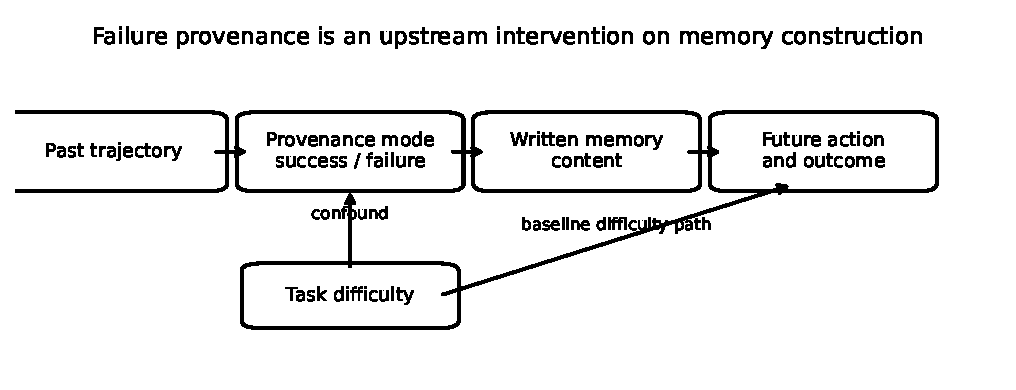
\includegraphics[width=\linewidth]{figures/fig1_provenance_causal.pdf}
\caption{Coarse causal structure of provenance-conditioned memory. Acquisition difficulty can affect both source outcome and later task performance. Writer mode mediates the path from source provenance to written memory; an optional visible provenance-metadata channel is omitted for readability. Matching future queries and semantic guidance reduces the task-difficulty confound but does not make generated memories identical.}
\label{fig:causal}
\end{figure}

\subsection{A provenance effect is not a single estimand}
The observational quantity
\begin{equation}
A_P = \mathbb{E}[Y\mid P=S]-\mathbb{E}[Y\mid P=F]
\end{equation}
is useful as an audit signal, but it is not causal: acquisition difficulty $D$ can influence both $P$ and future outcomes. More importantly, a notation such as $do(P)$ is underspecified once provenance controls memory construction. One must state which downstream channel is intervened on.

The \emph{writer-mode contrast} changes the reflection objective while fixing the future query and released observation state:
\begin{equation}
\Delta_W(x') =
\mathbb{E}[Y\mid do(W=W_F),x',E,\mathcal{G}=1]-
\mathbb{E}[Y\mid do(W=W_S),x',E,\mathcal{G}=1],
\label{eq:writer}
\end{equation}
where $E$ denotes the frozen future evidence/state and $\mathcal{G}$ is a preregistered information-equivalence gate on the two generated memories. This is the object approximated by our R4 and R6 bridges. Even when $\mathcal{G}=1$, the intervention can change wording, emphasis, decomposition, or other decision-relevant properties of $M$; therefore $\Delta_W$ is a writer-mode-bundle estimand, not automatically a provenance-metadata-only effect.

A stricter \emph{exact-information provenance-exposure contrast} holds actionable memory content, retrieval membership, and retrieval order fixed, and changes only whether truthful source-outcome provenance is visible to the executor. For a retrieved memory set $m$ with truthful provenance vector $p$, define
\begin{equation}
\Delta_L(m,x') =
\mathbb{E}[Y\mid M=m,do(L=p),x',E]-
\mathbb{E}[Y\mid M=m,do(L=\varnothing),x',E].
\label{eq:metadata}
\end{equation}
This is an incremental-information estimand: it asks whether exposing provenance adds value beyond the same actionable content, rather than assuming that SUCCESS or FAILURE has a fixed sign. Historical R5 targets the same rung but support-stops before model execution. The fresh R53--R57 experiment executes this contrast prospectively on 32 independent MemRL/OSInteraction clusters.

\subsection{Provenance-audit identification ladder}
Table~\ref{tab:ladder} turns these distinctions into a reusable audit protocol. The key reporting rule is that request count is not automatically the inference unit: R4 contains 48 completed requests but only four independent task units; R6 contains 276 requests but 23 independent task units.

\begin{table}[t]
\centering
\caption{Provenance-audit identification ladder.}
\label{tab:ladder}
\scriptsize
\begingroup
\setlength{\tabcolsep}{2pt}
\begin{tabular}{p{0.06\linewidth}p{0.34\linewidth}p{0.25\linewidth}p{0.25\linewidth}}
\toprule
Rung & Intervention / hold fixed & Current evidence and independent unit & Strongest allowed claim \\
\midrule
L0 & Observe provenance strata; no intervention & Financial audit; source/retrieval cases & Association / audit signal only \\
L1 & Switch writer mode; fix future query/state; require $\mathcal{G}=1$ & R4: 4 task pairs; R6: 23 task pairs & Writer-mode-bundle contrast, not provenance-only \\
L2 & Fix retrieval/content/order; hide vs expose truthful provenance & R56: 32 fresh paired clusters, 64/64 arms & Incremental terminal value of visible provenance on this substrate \\
L3 & Repeat L1/L2 in original model/runtime/source artifacts & Financial AgentDojo replication debt & Transport evidence only \\
\bottomrule
\end{tabular}
\endgroup
\end{table}

\subsection{Decision rule and completed L2 resolution}
The historical L1 gates use a frozen $|\Delta|\geq0.15$ relevance floor and task-level randomization tests; R4's four tasks imply minimum exact one-sided $p=1/16$, while R6 misses both magnitude and significance. The fresh L2 experiment separately freezes 32 paired clusters, an absolute practical-relevance floor of 0.15, a two-sided exact paired sign test, and a 100,000-resample paired-cluster bootstrap interval before the first primary treatment. It completes all 64 arms. The observed B-minus-A terminal effect is $0.03125$, with one B-only success, no A-only success, exact $p=1.0$, and preregistered bootstrap interval $[0,0.09375]$; the practical floor is not met. We therefore report qualified low incremental terminal value rather than a directional provenance benefit or a proof of exact zero.

\subsection{Identification statements}
Let $Y_W(w)=H(x',G(\tau,w),L_0,S)$ denote the potential outcome under writer mode $w$ with metadata fixed at $L_0$, and let $Y_L(\ell;m)=H(x',m,\ell,S)$ denote the potential outcome under provenance surface $\ell\in\{\varnothing,p\}$ with actionable memory set $m$ fixed exactly.

\paragraph{Proposition 1 (rung validity).} (i) L0 does not identify either $\Delta_W$ or $\Delta_L$ without an ignorability assumption for source provenance, because a latent acquisition difficulty can jointly affect $P$ and $Y$. (ii) Within a preregistered L1 admitted set, if writer mode is the only manipulated channel, future state $E$ is fixed, and consistency/no-interference hold, the paired task-level contrast identifies the finite-set writer-mode effect $\mathbb{E}[Y_W(W_F)-Y_W(W_S)]$ for that admitted set. (iii) L1 does not identify $\Delta_L$ when $G(\tau,W_F)\neq G(\tau,W_S)$. (iv) Under L2, if retrieved actionable content is byte-identical, retrieval membership/order are fixed, and executor-visible provenance is the only manipulated channel, the paired task-level contrast identifies $\mathbb{E}[Y_L(p;m)-Y_L(\varnothing;m)]$ for the evaluated substrate. L3 changes the target domain, not the intervention channel, so transport assumptions are additional to (ii)--(iv).

The non-upgrade in (iii) is constructive: two response functions can agree on every L1-observed point $(M_S,L_0)$ and $(M_F,L_0)$ yet differ arbitrarily on the unobserved metadata counterfactuals $(m,L_S)$ and $(m,L_F)$. Thus no amount of L1 replication alone determines an L2 effect. For our L1 gate, malformed memories, answer leakage, insufficient embedding similarity, verifier-detected actionable asymmetry, or a unique task-solving fact are rejected before outcomes; this narrows the writer-mode bundle but does not supply the missing equality assumption. Consequently a strong L0 signal cannot be promoted to L1/L2, a non-decisive L1 result cannot rescue L2, and an L2 support failure is not counterevidence. The rung and independent unit are therefore part of the claim, not bookkeeping.

\section{Released Evidence for a Provenance Effect}
\label{sec:evidence}
We begin from the public aggregate audit of ReasoningBank on benign AgentDojo Banking endpoints \citep{li2026audit}. The audit separates retrievals according to whether the retrieved memory was derived from a successful episode or from a failed episode. Table~\ref{tab:provenance} reproduces the reported counts after converting the rounded accuracies back to their integer support.

\begin{table}[t]
\centering
\caption{Provenance-conditioned ReasoningBank outcomes from the released financial-agent audit.}
\label{tab:provenance}
\small
\begin{tabular}{lrrr}
\toprule
Retrieved memory provenance & Cases & Correct & Accuracy \\
\midrule
Success-derived & 101 & 94 & 0.931 \\
Failure-derived & 34 & 22 & 0.647 \\
\bottomrule
\end{tabular}
\end{table}

The observed accuracy gap is 28.4 percentage points. This is a large effect at the retrieval stratum level. The transition audit gives the provenance signal a sharper interpretation. ReasoningBank records 25 W$\rightarrow$C recoveries and 9 C$\rightarrow$W regressions. Ten W$\rightarrow$W persistent failures remain after evolution. All ten belong to the failure-derived retrieval stratum.

The rounded provenance accuracies imply 12 failures among 34 failure-derived retrievals and 7 failures among 101 success-derived retrievals. The ten W$\rightarrow$W cases therefore account for roughly 83.3\% of failures in the failure-derived stratum. The success-derived stratum contains no W$\rightarrow$W case in the audit. Figure~\ref{fig:source} visualizes this decomposition.

\begin{figure}[t]
\centering
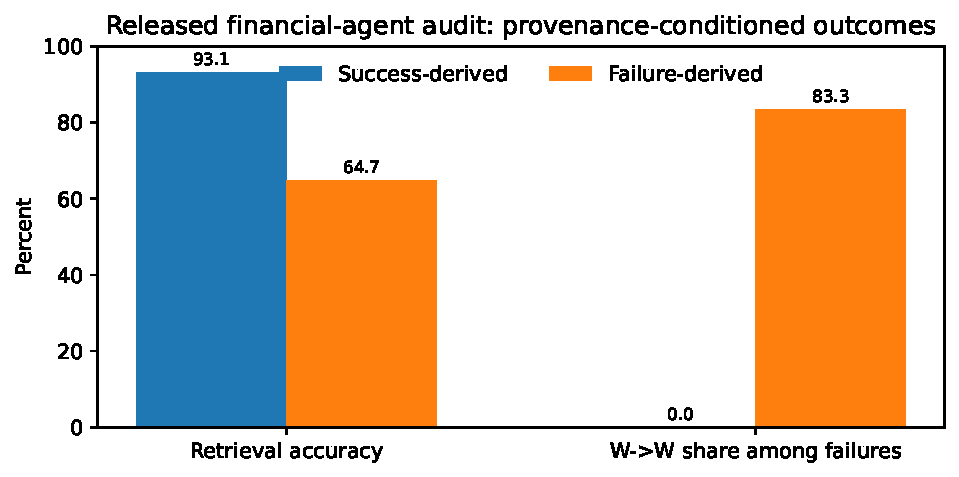
\includegraphics[width=0.95\linewidth]{figures/fig2_source_reanalysis.pdf}
\caption{The released audit shows a large accuracy gap by memory provenance. Persistent W$\rightarrow$W failures are concentrated in failure-derived retrievals.}
\label{fig:source}
\end{figure}

\subsection{The signal is strongest for persistence}
The transition structure changes the scientific interpretation of the aggregate accuracy gap. Failure-derived memory is tightly associated with errors that persist across self-evolution. The source audit identifies task difficulty as a confound for this association. Our causal formulation preserves the persistence signal as the main target and removes task difficulty through an intervention on memory provenance.

A simple arithmetic check sharpens the motivating association. The failure-derived stratum contains roughly two failures beyond the ten W$\rightarrow$W cases, whereas the success-derived stratum contains seven failures. The provenance signal therefore concentrates on persistent error much more strongly than on newly induced regression. We treat this pattern as a reason to audit provenance, not as evidence that failure provenance itself causes persistence.

\subsection{Independent mechanism evidence}
Memory Reward Inflation studies a different memory architecture and identifies an amplification channel for erroneous memories \citep{asadolahi2026inflation}. Incorrect memories can receive inflated utility scores, which increases their future reuse, including under similarity-based retrieval. This illustrates why observed memory reward, retrieval frequency, and source provenance can become entangled. It does not predict a fixed success/failure provenance sign.

Together, the financial-agent audit and reward-inflation results motivate a causal audit of what information provenance contributes beyond memory content. Section~\ref{sec:intervention} first localizes the writer-mode bundle with historical L1 endpoints and then executes the exact-information L2 provenance-exposure contrast.

\section{Controlled Evidence Across Writer and Provenance Channels}
\label{sec:intervention}
The controlled evidence separates two channels that are often conflated. Historical L1 experiments change an outcome-conditioned memory writer and therefore identify a writer-mode bundle. Our main L2 experiments instead hold retrieval membership, order, and actionable memory bytes fixed and change only whether an explicit truthful source-outcome indicator is masked or revealed to the executor. The masked arm can still contain implicit outcome clues in the memory text; the treatment therefore measures incremental field exposure beyond content, not provenance-versus-no-provenance.

\subsection{Historical L1 bridge}
Two preregistered WebArena bridges motivate the cleaner intervention but do not identify provenance alone. A terminal-success experiment admits four information-equivalent task pairs and completes 48 requests; the success-writer minus failure-writer effect is $+0.1667$ with $p=0.0785$. With only four independent tasks, the smallest exact one-sided sign-flip value is $1/16=0.0625$, so this endpoint is structurally non-decisive under the frozen 0.05 rule. A disjoint early-action experiment admits 23 task pairs and completes 276 requests; its reference-action-match effect is $-0.0942$ with counterevidence-side $p=0.0792$. The two estimands have opposite descriptive signs, and deterministic audits show systematic writer-style differences. We therefore make no endpoint-robust directional L1 claim and never upgrade L1 to provenance-only L2. Full admission rules, pair construction, runtime repair boundaries, tables, and randomization contracts are retained in Appendix~A.2--A.9.

\subsection{Fresh L2 provenance-exposure experiment}
\label{sec:l2fresh}
The main experiment is a new prospective treatment-outcome object and does not reuse historical R4/R6 outcomes or the stopped R5/R19 prefixes. Its source-bank capacity is nevertheless pilot-informed: an earlier 128-source support stop and zero-outcome diagnostic exposed coverage sensitivity, after which we chose the entire frozen 350-task training universe rather than tuning a smaller cutoff. The R53 lineage then rebuilds all 350 memories from zero under Qwen2.5-7B-Instruct and MemRL, one durable memory at a time. Fresh target selection excludes every historical validation signature and occurs before any new validation outcome. The source run completes 350/350 units with 176 success-derived and 174 failure-derived memories. This balance is descriptive; source outcomes are never used to choose target units.

Before any validation environment is reset, we apply native MemRL retrieval ($k=10$, cosine threshold $0.5$) to fresh exact skill-signature clusters from the frozen validation split. All 40 historical primary/utilization signatures are excluded. Of 108 remaining clusters, 106 have at least one eligible retrieved memory with nonempty content, a source task in the full source universe, and a boolean source outcome. Frozen hash ranking selects the first 32 eligible clusters as the primary sample and the next eight as a disjoint utilization sample. No target outcome is observed during this support step.

\paragraph{Utilization first stage.}
The eight utilization clusters each receive five frozen surfaces: no memory (U0), true retrieved memory (U1), null content (U2), reversed content (U3), and shuffled other-task memory (U4). Promotion uses only the first executable action; terminal success is diagnostic. U1 produces a first-action change relative to both U0 and U2 in 5/8 units, while U2 differs from U0 in 3/8. This satisfies the preregistered rule $5\geq3$ and $5\geq3+1$, rejecting the trivial explanation that the entire memory surface is inert before the primary contrast is opened. It is an anti-inertness guard, not proof that the executor semantically interprets the later source-outcome field.

\paragraph{Primary A/B contrast.}
For each of the 32 fresh primary clusters, the frozen retrieval is rendered into two executor views. In A, the explicit source-outcome field is masked while the retrieved content remains visible. In B, the same rows, order, and actionable content additionally reveal the truthful boolean \texttt{source\_outcome\_success} for each row. Similarity, Q estimates, scores, roles, memory IDs, and source task IDs are hidden from both arms; retrieval is not rerun between arms. Arm order is frozen per cluster before treatment. Each arm constructs a fresh task/session, calls \texttt{task.reset(session)} before inference, and OSInteraction's reset constructs a new Docker container with \texttt{remove=True}; \texttt{task.release()} runs in a \texttt{finally} path and terminates any remaining container. Thus task-visible filesystem/user/process state is arm-local. We hold the reset initial environment and feedback mechanism fixed, not realized downstream observations after actions diverge. All 64 Qwen arm runs complete without execution failure.

\begin{table}[t]
\centering
\caption{Fresh L2 terminal-success result. The inference unit is the paired dependency cluster.}
\label{tab:l2fresh}
\small
\begin{tabular}{lrr}
\toprule
Quantity & Outcome field masked (A) & Truthful outcome field revealed (B) \\
\midrule
Terminal successes & 15/32 & 16/32 \\
Success rate & 0.46875 & 0.50000 \\
\midrule
Paired $B-A$ effect & \multicolumn{2}{c}{$+0.03125$} \\
B-only / A-only successes & \multicolumn{2}{c}{1 / 0} \\
Exact two-sided sign test & \multicolumn{2}{c}{$p=1.0$} \\
Paired bootstrap 95\% interval & \multicolumn{2}{c}{$[0,0.09375]$} \\
Preregistered relevance floor & \multicolumn{2}{c}{$|\Delta|\geq0.15$; not met} \\
\bottomrule
\end{tabular}
\end{table}

Thirty-one of 32 pairs have identical terminal outcomes. The only discordant pair favors B, but one discordant unit supplies essentially no directional resolution under the exact two-sided paired test; $p=1.0$ is not affirmative evidence for zero effect. The preregistered bootstrap interval is reported as specified; because the empirical paired-effect distribution contains 31 zeros and one $+1$, we do not interpret its upper endpoint as an equivalence bound. A post-confirmatory conservative paired-risk-difference audit separately gives $[-0.128,0.183]$, so a $+0.15$ population effect is not excluded. The supported statement is therefore descriptive and threshold-based: the observed $+3.125$-point effect did not reach the preregistered 15-point threshold on the frozen 32-pair sample.

\paragraph{Local policy sensitivity and a real Task~252 example.}
A complete-run diagnostic shows that A and B differ in first executable action for 9/32 clusters and in total step count for 7/32, while terminal success differs for only 1/32. This establishes local sensitivity to the field-exposure treatment, but it does not distinguish semantic use of source outcome from generic structured-prompt sensitivity. The binary terminal endpoint is also many-to-one: behaviorally different trajectories can reconverge after later OS feedback and receive the same success label.

The sole Qwen terminal-discordant cluster is OSInteraction Task~252: \emph{create user \texttt{appuser}, create \texttt{/home/appuser/config.cfg} with \texttt{DEBUG\_MODE=true}, and set mode 600}. Its frozen retrieval contains five memories in the same order in both arms: source tasks 74, 403, 208, and 210 are success-derived configuration/user/permission examples; source task 450 is a failure-derived reflection whose visible text already recommends checking environment capabilities, errors, permissions, and ownership. Thus A is not provenance-information-free. Qwen A takes 16 steps and fails; Qwen B, with only the explicit truthful outcome fields added, takes 8 steps and succeeds after adapting to missing \texttt{sudo} and interactive-\texttt{vi} problems. Under Llama, the same Task~252 A/B surfaces yield different first actions but both succeed in 5 steps. We use this outcome-selected case only to illustrate one possible closed-loop pathway; it is not evidence that semantic provenance reasoning explains the aggregate treatment effect.

\subsection{Executor-backbone replication}
\label{sec:l2replication}
To test whether the low-terminal-value pattern is specific to the Qwen executor, we freeze a second prospective experiment before any Llama validation outcome. It reuses the same 350-memory source bank, R54 frozen retrieval membership/content/order, eight utilization clusters, 32 primary clusters, exact-information renderer, terminal evaluator, randomization rule, and complete-only analysis. Importantly, the source memories themselves were written once by the Qwen/MemRL source process and are reused unchanged; this is therefore an executor-backbone replication, not an independent writer- or retriever-backbone replication. The only scientific factor changed at evaluation is the executor, from Qwen2.5-7B-Instruct to Meta-Llama-3.1-8B-Instruct. A source-side native parser qualification passes 3/3 before validation exposure.

The Llama utilization first stage also passes rather than borrowing the Qwen qualification: true memory produces the required memory-specific first-action divergence in 8/8 clusters, while null-memory versus no-memory differs in 5/8, satisfying $8\geq3$ and $8\geq5+1$. Thus a low terminal A/B contrast cannot be dismissed as complete memory-channel inertness, although the placebo divergence also cautions that first-action sensitivity alone does not prove semantic provenance use. All 64 Llama primary arms complete exactly once.

\begin{table}[t]
\centering
\caption{Exact-information L2 results by executor backbone. Models are adjudicated separately; no cross-model pooling is performed.}
\label{tab:l2backbones}
\scriptsize
\begin{tabular}{lrrp{0.34\linewidth}}
\toprule
Executor & $B-A$ & Discordant & 95\% intervals: preregistered bootstrap; conservative paired RD \\
\midrule
Qwen2.5-7B-Instruct & $+0.03125$ & 1/32 & $[0,0.09375]$; $[-0.128,0.183]$ \\
Meta-Llama-3.1-8B-Instruct & $0.00000$ & 4/32 & $[-0.125,0.125]$; $[-0.225,0.225]$ \\
\bottomrule
\end{tabular}
\end{table}

For Llama, two clusters are B-only successes and two are A-only successes, so the observed paired terminal effect is exactly zero and the discordances are directionally balanced. The exact sign test remains $p=1.0$ for both models (omitted from the table for space), but sparse discordance makes that value low-resolution rather than affirmative null evidence. Table~\ref{tab:l2backbones} therefore reports both the frozen bootstrap and the post-confirmatory conservative paired-risk-difference audit. Neither observed point estimate reaches the preregistered $|\Delta|\geq0.15$ threshold, yet neither conservative interval establishes $\pm0.15$ equivalence or excludes a $+0.15$ population effect. The model-specific results are not combined. The replication is correspondingly narrow: local action sensitivity with sparse terminal discordance recurs under a second executor on the same source-bank/retrieval/task/renderer substrate.

\paragraph{L3 transport.} A source-faithful test still requires the motivating financial writer/checkpoint, original memory interface, fixed acquisition content, and paired source runtime; WebArena or MemRL is not a substitute. Appendix~\ref{app:l3} gives the transport contract. L3 therefore remains replication debt.

The replicated L2 result sharpens a limited governance implication. An explicit source-outcome field can alter local action selection, but the observed terminal estimates on these frozen samples do not reach the prespecified 15-point threshold and do not establish an automatic positive trust value. Section~\ref{sec:psmg} therefore treats provenance as auditable control-plane information whose decision weight must be independently justified, rather than as a monotone SUCCESS/FAILURE trust rule. Neither R56 nor the Llama replication tests PSMG efficacy.

\section{Provenance-Separated Memory Governance}
\label{sec:psmg}
The identification result suggests a governance response that does not guess the sign of provenance. Let a memory record be
\begin{equation}
r_i=(m_i,p_i,z_i,h_i),
\end{equation}
where $m_i$ is actionable content, $p_i$ process provenance, $z_i$ all other pre-outcome quality/relevance features, and $h_i$ a content-addressed audit pointer. PSMG keeps $(p_i,h_i)$ in the control plane instead of silently deleting provenance or concatenating it to every executor prompt.

\paragraph{Calibrated decision and executor-blind projection.}
A frozen controller $g_\theta(z_i,p_i)$ selects admit, down-weight, verify, or withhold; failure-derived memory is never rejected by definition. A projection $\Pi$ then sends only approved actionable content (plus separately authorized verification evidence) to the executor, keeping raw $p_i$ hidden unless executor-facing provenance is itself the declared treatment. This separates governance value from a lexical provenance cue and allows provenance influence to shrink toward zero when conditional information gain is unsupported.

\paragraph{Same-information efficacy test.}
The decisive comparator is $g^0_\phi(z_i)$, which receives every pre-outcome feature available to PSMG except $p_i$. Memory bytes, support, retrieval/content budget, executor, verification information, task distribution, endpoint, and analysis must remain fixed. Only an advantage over this comparator identifies decision value attributable to provenance in the governance plane. Our L2 experiments instead test executor-visible $Y_L(p;m)-Y_L(\varnothing;m)$, so PSMG remains a prospective method design rather than an efficacy claim (Appendix~\ref{app:fresh}).

\section{Related Work}
\paragraph{Agent memory, provenance, and trust.} A-MEM and MemRL organize or score reusable memories by content and utility, while ReasoningBank, Agent Workflow Memory, and Reflexion turn trajectories or feedback into persistent state \citep{xu2025amem,zhang2026memrl,ouyang2026reasoningbank,wang2024awm,shinn2023reflexion}. Provenance is also established as a governance object: execution-tracing work records evidence lineage \citep{wang2026tracetotrust}, Memory Provenance Laundering studies source-authority loss under consolidation \citep{xu2026laundering}, and MutMem binds outcome evidence to authorized memory mutation \citep{saidi2026mutmem}. We therefore claim neither provenance storage nor trust scoring as a new primitive.

\paragraph{Provenance-bearing architectures and failure-derived experience.} Eywa links derived beliefs to immutable source evidence, TierMem links lossy summaries to raw pages, and MemORAI tracks turn-level origins in a provenance-enriched graph \citep{joshi2026eywa,zhu2026tiermem,pham2026memorai}. These systems make provenance operational, but changing a summary route, graph edge, or writer can also change actionable information. Separately, Learning from Failure, multi-round skill evolution, and Experiential Reflective Learning show that failure-derived experience can be useful, while Memory Reward Inflation shows that erroneous memories can also be amplified \citep{sun2026learningfromfailure,liu2026rethinkingfeedback,allard2026erl,asadolahi2026inflation}. Hence source failure has no justified universal trust sign.

\paragraph{Identification-to-governance boundary.} The financial-agent audit supplies a strong success/failure provenance association \citep{li2026audit}, but task difficulty can confound it. Our L0--L3 ladder separates observation, writer-mode intervention, byte-identical metadata intervention, and source transport before assigning a claim. PSMG then uses that separation architecturally: provenance stays in auditable control-plane state, executor-visible content is separated from the raw provenance cue, and the decisive comparator receives the same non-provenance information. The closest primitives above can implement pieces of this design; the paper-level distinction is the coupling of rung-specific identification to a same-information governance test. That test remains future work, so PSMG is not presented as a validated performance improvement.

\section{Limitations}
The motivating financial audit lacks the per-query artifacts and auditable model/interface bindings required for source-faithful L3 transport. Our completed L2 evidence instead uses one MemRL/OSInteraction source bank with two executors, so the result is model-robust within this frozen information surface rather than a universal provenance theorem. The full-350 source capacity was chosen after a zero-outcome diagnosis of an earlier 128-source support stop; it should therefore be understood as pilot-informed capacity design, while the subsequent source rebuild, fresh disjoint target selection, treatment schedule, and target outcomes are prospective. The Llama study also reuses the Qwen/MemRL-generated source memories and frozen retriever outputs, so it isolates executor-backbone robustness rather than writer or retrieval robustness. Historical L1 bridges remain writer-mode-bundle evidence because information identity is imperfect; stopped R5/R19/R51 objects remain fail-closed and are never pooled with the fresh lineage (Appendix~A.2--A.12).

The fresh estimates are also finite and terminal discordance is sparse. Qwen gives an observed $\Delta=+0.03125$ with one discordant pair and preregistered bootstrap interval $[0,0.09375]$; Llama gives an observed $\Delta=0$ with four discordant pairs and preregistered interval $[-0.125,0.125]$. Neither point estimate reaches the prespecified 0.15 threshold. However, a post-confirmatory conservative paired-risk-difference audit gives Qwen $[-0.128,0.183]$ and Llama $[-0.225,0.225]$, so the present data do not establish $\pm0.15$ equivalence or rule out a $+0.15$ population effect. The exact $p=1.0$ values are correspondingly low-resolution under sparse discordance, not affirmative evidence for zero. First-action differences show treatment sensitivity, but because adding the structured field changes prompt surface as well as information, they do not by themselves prove semantic provenance reasoning. PSMG efficacy is likewise untested because L2 exposes an outcome field to the executor rather than comparing a provenance-sensitive governor with a strongest same-information provenance-free controller.

\section{Conclusion}
The L0--L3 ladder separates provenance association, outcome-conditioned writer effects, explicit source-outcome-field exposure, and source-faithful transport. Once retrieved memory content is fixed, the large motivating association does not reproduce as a comparably large \emph{observed} terminal difference in the frozen samples: Qwen yields $+3.125$ percentage points and Llama $0$, and neither point estimate reaches the preregistered 15-point threshold. At the same time, the conservative sparse-discordance intervals remain wide enough that this is not a practical-equivalence result. Explicit field exposure changes first-action selection in 9/32 Qwen and 8/32 Llama pairs, while the closed-loop environment and binary evaluator often absorb those differences before the terminal label. The defensible conclusion is therefore narrower: this structured source-outcome cue has clear local policy effects but limited observed aggregate terminal impact on the shared frozen OSInteraction surface; semantic provenance value in general remains unresolved.

The engineering implication is not to discard provenance, but to stop treating SUCCESS/FAILURE as an automatic trust score. PSMG preserves lineage for audit and lets a calibrated governor use it only when it adds information beyond content and context. A format-matched semantic-control experiment---for example UNKNOWN/masked versus truthful versus reversed/shuffled values with the same field present in every arm---would be the highest-information extension for separating semantic outcome information from generic structured-prompt sensitivity. Source-faithful L3 transport and a prospective PSMG-versus-same-information-controller trial remain separate open tests.


\section*{Reproducibility Statement}
The appendix records frozen intervention, inference, and support-failure rules. The supplement binds the claim ledger, evidence receipts, and rebuildable source to content-addressed artifacts.

\section*{AI Use Disclosure}
LLM tools assisted literature triage, implementation, analysis, editing, and mock review. Claims and numbers were checked against frozen artifacts and deterministic scripts; AI judgments were not task-success ground truth. The authors take responsibility for the final content.

\bibliography{references}
\bibliographystyle{iclr2027_conference}
\appendix
\section{Source-Grounded Reanalysis and Intervention Details}
\subsection{Count reconstruction}
The financial audit reports 101 success-derived retrievals at 0.931 accuracy and 34 failure-derived retrievals at 0.647. The unique integer numerators consistent with three-decimal rounding are 94 and 22, yielding 7 and 12 failures. It also reports ten W$\rightarrow$W persistent failures, all failure-derived; hence 10/12 failure-derived errors are persistent, while the success-derived stratum contains no W$\rightarrow$W case.

\subsection{Terminal information-equivalence contract}
Six terminal candidates are frozen before outcomes. Both memories use the same writer model; eligibility requires valid ReasoningBank items, paired embedding cosine at least 0.75, an independent verifier judging actionable guidance equivalent with no unique task-solving fact, and no literal benchmark-reference leakage. Four candidates pass: tasks $\{387,167,23,388\}$ with cosines 0.931, 0.902, 0.906, and 0.904. The same four remain eligible if the cosine floor is raised from 0.75 to 0.85 or 0.90; this is a zero-call re-thresholding of archived pre-outcome values, not an alternative-verifier run. Task 385 is excluded for repeating ``Cally''; task 164 repeats ``Dry'' and ``Uneven color.'' All exclusions are pre-outcome.

\subsection{Post-hoc operational-equivalence stress test}
The original information-equivalence gate remains the preregistered R4 admission rule; the following diagnostics do not retroactively change eligibility. An archived stronger-verifier audit judges none of the four admitted R4 pairs fully equivalent under one semantic reviewer and only one of four fully equivalent under a second, with the residual disagreements involving concrete strategy emphasis. A deterministic lexical audit points in the same direction without a new model call: failure-derived memory contains more search/filter language and more strong-directive language in all 6/6 R4 writer pairs; among the 24 R6 writer pairs it contains more failure/caution language in 23/24, more verification language in 20/24, and more strong-directive language in 20/24. These diagnostics make the limitation operational: the success/failure ReasoningBank intervention changes writer mode together with pragmatic register and strategy emphasis. They therefore weaken a provenance-only interpretation of L1 and increase the value of the byte-identical L2 intervention; they do not change either frozen L1 outcome.

\subsection{Terminal runtime repair boundary}
A condition-blind projection removes repeated global menu blocks, blank lines, and exact duplicate lines without consulting references or outcomes. An initial context-allocation support failure is discarded before scientific admission; the clean restart changes only context capacity. Its largest prompt uses 5,209 of 12,288 input tokens; executor, temperature, seed schedule, pair set, scorer, effect floor, permutation seed, and significance rule remain frozen.

\subsection{Terminal statistical rule}
Each qualified pair receives six paired seeds. The statistic is task-level terminal success, success-derived minus failure-derived. Support requires $\Delta\geq0.15$ and one-sided $p<0.05$; counterevidence requires $\Delta\leq-0.15$ and its one-sided $p<0.05$, using 100,000 frozen-seed permutations. Observed $\Delta=+0.1667$ with $p_S=0.0785$. Four independent task units imply only 16 exact sign assignments and a minimum one-sided value $1/16=0.0625$, so this endpoint cannot satisfy the frozen $0.05$ rule.

\subsection{Early-action cohort and L1 writer-mode contrast}
The disjoint WebArena cohort excludes prior D2 task IDs. A candidate must come from a released successful trajectory and expose a visible single-click reference action at step two or later; eligible tasks are sorted by ID and the first 24 are frozen before counterfactual writing. A compact process trace preserves instruction and action sequence but removes terminal success. The same trace is passed through first-party ReasoningBank success- and failure-reflection prompts using Qwen2.5-32B at temperature zero, directly varying outcome-conditioned writer mode while holding the trace fixed.

Eligibility again requires valid memory items, cosine at least 0.75, verifier-equivalent actionable guidance, no unique task-solving fact, and no reference-action leakage. Twenty-three pairs pass; candidate 159 is excluded for an unparsable verifier output. All 23 enter downstream execution.

\subsection{Early-action statistical rule}
Each task receives six paired seeds per writer condition with identical future query and frozen browser state. The output is one visible click index; the released successful trajectory supplies the reference. Inference is task-level: the permutation test sign-flips each task's success-derived minus failure-derived reference-match difference over 100,000 draws, with the same $\pm0.15$ magnitude and one-sided $0.05$ gates. The 23 tasks yield 276 complete requests and zero support failures; mean difference is $-0.0942$, with $p_S=0.9841$ and $p_F=0.0792$. Paired actions differ in 21.0\% of seeds; hypothesis-direction error-consistent divergence is 0.7\%, versus 10.1\% in reverse.

\subsection{Exact-information support-capacity stop and reopen condition}
R5 holds the actionable memory core byte-identical and changes only structured provenance metadata. Its frozen contract requires ten unique review tasks, but the released shopping split contains only five; it therefore stops before any model call, with no scientific verdict and no post-audit target reduction. The strongest reopen path is source-faithful financial AgentDojo replication of an L1 writer-mode or L2 exact-information contrast when query-level artifacts or auditable exact-model access become available. Such replication addresses L3 transport, not identification by itself; any new bridge must be frozen before outcomes and cannot reuse R4/R6 for threshold rescue.

\subsection{Prospective L1 power-planning contract}
\label{app:power}
The current $|\Delta|\geq0.15$ rule is a practical-relevance floor, not evidence of adequate power. A future confirmatory L1 run must choose the number of independent task pairs before outcomes by simulation or exact enumeration of the planned task-level sign-flip test. The planning distribution must be frozen from an external pilot or other prespecified source; the target effect is $|\Delta|=0.15$; the directional randomization threshold remains 0.05; and the target prospective power is at least 80\%. Pair construction, task exclusions, seeds per condition, maximum task count, and the stopping rule must be frozen with that calculation. Repeated requests within a task may reduce task-level measurement noise but do not count as additional independent units.

For scale, a normal-approximation planning sensitivity for a paired task-level mean at $|\Delta|=0.15$ gives the following independent-task counts. These are design aids, not retroactive evidence, because the unknown task-level standard deviation must be fixed prospectively from an external pilot.
\begin{center}
\begin{tabular}{lrr}
\toprule
Planning SD & one-sided $\alpha=.05$, 80\% power & two-sided $\alpha=.05$, 80\% power \\
\midrule
0.20 & 11 & 14 \\
0.30 & 25 & 32 \\
0.40 & 44 & 56 \\
\bottomrule
\end{tabular}
\end{center}
Thus ``four tasks'' is not defended as an adequately powered design; even the optimistic SD=0.20 planning case points to a double-digit confirmatory cohort. R4 remains structurally non-decisive, and R6 is judged by its frozen effect and significance gates rather than post-hoc sample extension. We retain the preregistered directional randomization tests as the decision tests. A future confirmatory packet should additionally report a two-sided randomization sensitivity and a paired confidence interval; BCa intervals are descriptive rather than a substitute for the frozen randomization gate, and are not retrofitted onto the four-task R4 endpoint.

\subsection{Source-faithful L3 decision contract}
\label{app:l3}
An L3 transport test must recover the motivating financial-agent writer/checkpoint and original memory interface, freeze the same acquisition trajectory content and downstream schedule across conditions, and manipulate only the declared provenance channel before any outcome is observed. For an L1 source-native test, success- versus failure-conditioned writer mode may change the generated memory, after which the pre-outcome information-equivalence audit is applied and the paired memories are executed in the original runtime. For an L2 source-native test, actionable memory, retrieval membership, and retrieval order must remain fixed while only executor-visible provenance information changes (e.g., truthful provenance hidden versus exposed).

The current obstacles separate cleanly. \emph{Infrastructure debt} is the missing query-level ReasoningBank artifacts, auditable access to the reported Qwen 3.7 Flash writer and qwen3.7-text-embedding configuration, source checkpoint/prompt bindings, and provenance-bearing runtime fields needed to replay the original financial tasks. \emph{Conceptual requirements} remain even after those assets exist: the intervention channel must be declared before outcomes; L1 must retain a pre-outcome information-equivalence gate; L2 must keep actionable memory byte-identical; and any WebArena-to-financial transport claim must state its target-population assumptions rather than treating source replication as automatic generalization. A writer-output change plus downstream change supports a source-native writer-mode path; a byte-identical-memory metadata contrast with downstream change supports an L2 metadata path on that substrate; and adequate-support null evidence on both channels is substrate-bounded counterevidence rather than a general no-provenance theorem. No such source-faithful execution is claimed in the present paper.

\subsection{Fail-closed R19 stop and non-reuse rule}
A later L2 compatibility experiment prospectively freezes 35 independent tasks and 140 terminal episodes under a two-sided task-level sign-flip primary analysis. It reaches 29/140 durable episodes: seven tasks are complete and one episode of an eighth task is complete. The next reset then times out before STARTED; the single exact pre-exposure retry allowed by the frozen contract also times out before STARTED. Because the retry budget is exhausted, the confirmatory attempt stops. No task-level deltas, effect mean, $p$-value, interval, or subgroup result is computed from the partial prefix for manuscript claims. The prefix may not be pooled into a later cohort and may not select a new threshold, endpoint, model, controller, or statistical rule.

After excluding every template exposed by the stopped attempts, the same frozen asset contains 27 fully unexposed templates. This is inventory, not an automatically authorized replacement cohort. For reference, the preregistered planning sensitivity at task-level SD $0.30$ requires about 32 independent tasks for a two-sided 80\% target at $|\Delta|=0.15$; $n=27$ is below that reference. Sample scarcity is therefore not a reason to lower the gate.

\subsection{Fresh R53--R57 L2 execution contract and receipts}
The completed L2 experiment is a new lineage rather than a continuation of R19. R53 executes all 350 tasks in the frozen OSInteraction training split under a single exactly-once source-memory attempt, producing 176 success-derived and 174 failure-derived memories. Its source receipt records 350/350 completed units and zero external-provider calls. R54 evaluates retrieval support before any validation environment reset. Historical validation signatures are excluded; among 108 fresh exact skill-signature clusters, 106 have eligible native retrieval. Hash ranking freezes 32 primary and eight utilization representatives before the first validation treatment.

R55 then executes 40 utilization arms (eight clusters times five memory surfaces) with started/completed durability ledgers. It completes 40/40 without failure. The frozen promotion rule uses the first executable action only: true memory is specifically divergent from both no-memory and null-memory in 5/8 clusters, versus 3/8 null-memory versus no-memory divergences, so the first stage passes. Terminal success in R55 is diagnostic and is not used to select the primary sample.

R56 freezes the A/B schedule before its first treatment. The R39 exact-information adapter renders each selected retrieval into A (explicit source-outcome field masked) and B (the same rows/content/order plus truthful boolean source outcome). The adapter audit requires actionable-content identity and verifies that \texttt{source\_outcome\_success} is the only executor-visible field added in B; similarity, Q values, scores, IDs, and source task IDs are hidden. Memory text itself is not scrubbed of implicit outcome clues, so A is a masked-field baseline rather than a no-provenance-information condition. All 64 arms complete with zero execution failures. Complete-only analysis yields A=15/32, B=16/32, observed $\Delta=0.03125$, one discordant pair, exact two-sided sign-test $p=1.0$, and the frozen 100,000-resample paired bootstrap interval $[0,0.09375]$. The observed effect does not reach the 0.15 threshold; no equivalence claim is implied.

\subsection{R59--R62 executor-backbone replication}
The second-backbone experiment is prospectively frozen after R57 and before any Llama validation outcome. The local Meta-Llama-3.1-8B-Instruct artifact is content-addressed, and a 3/3 source-side native-parser qualification passes without opening validation or terminal outcomes. The replication then reuses the exact R54 source bank and frozen retrieval content/order, the same eight utilization and 32 primary cluster IDs, the same R39 exact-information A/B renderer, and the same evaluator/randomization/analysis; only the executor backbone changes.

R60 executes 40 Llama utilization arms and completes 40/40 without failure. The memory-specific first-action criterion holds in 8/8 clusters, while null-memory versus no-memory differs in 5/8, so the frozen promotion gate passes before any primary outcome. R61 then executes the 64 frozen A/B arms exactly once. Complete-only analysis gives an observed $\Delta=0$, two B-only and two A-only successes, four discordant pairs, exact two-sided sign-test $p=1.0$, and the frozen 100,000-resample paired bootstrap interval $[-0.125,0.125]$. The observed effect does not reach the 0.15 threshold. R62 adjudicates Qwen and Llama separately, without statistical pooling. This is executor-only robustness within one shared source-bank/retrieval/task/renderer substrate, not an independent pipeline replication or universal zero-effect claim.

\subsection{R66 post-confirmatory sparse-discordance and isolation audit}
R66 changes no experimental outcome, threshold, frozen analysis, or execution authority. First, it adds a conservative paired-risk-difference audit for the sparse binary discordances. Let $p_{10}=P(B=1,A=0)$ and $p_{01}=P(B=0,A=1)$, so the paired risk difference is $p_{10}-p_{01}$. We form separate exact two-sided 97.5\% Clopper--Pearson intervals for $p_{10}$ and $p_{01}$ and combine them by Bonferroni as $[L_{10}-U_{01},U_{10}-L_{01}]$, guaranteeing at least 95\% simultaneous coverage. This yields Qwen $[-0.128,0.183]$ and Llama $[-0.225,0.225]$. Consequently neither model establishes $\pm0.15$ equivalence and neither conservatively excludes a $+0.15$ population effect. These intervals are a post-confirmatory wording audit and do not replace the preregistered bootstrap/sign test.

Second, R66 audits arm isolation at the bound implementation. The shared \texttt{run\_arm\_exact} creates a fresh task and session per arm, invokes \texttt{task.reset(session)} before the inference loop, and invokes \texttt{task.release()} in a \texttt{finally} block. At pinned MemRL revision \texttt{c1b322ca}, OSInteraction reset constructs a new \texttt{OSInteractionContainer}; its container constructor launches a fresh Docker container with \texttt{remove=True}, while normal completion and release terminate the container. Thus one arm is not intended to inherit task-visible users, files, or processes from the preceding arm. The experiment holds the reset initial environment-generation mechanism fixed; once treatment changes an action, later observations are permitted to differ as treatment-induced mediators. The original ledgers do not contain a dedicated per-arm \texttt{reset\_success} timestamp bit, so the audit is code-level reset/container evidence plus 64/64 completed-arm evidence rather than a newly manufactured runtime receipt.

\subsection{Future transport and governance gate}
\label{app:fresh}
L3 transport or PSMG-efficacy evaluation remains a new scientific object and opens only after its treatment-independent components are frozen. For PSMG efficacy, the provenance-sensitive controller, strongest same-information provenance-free comparator, calibration data, decision thresholds, and action mapping must be executable and content-addressed before target outcomes. For L3, the motivating source runtime and artifacts must be recovered. The completed Qwen and Llama L2 results remain fixed regardless of future experiment direction and may not be reinterpreted as failed attempts to be rescued.

\end{document}
